\chapter{Implementation and Evaluation}
\noindent

	In this chapter, we will introduce our proposed system that includes five core components processing HC images and estimate the perimeter of the fetus' head. Each of the components is an restful API which works on specific task (inspired from micro service design). Therefore, in the future, we can easily scale up the number of workers (API) to speed up the process and manage them more conveniently in the deployment phrase. For more details, the system's design is shown in \ref{fig:hc_system}.
	
	\begin{figure}[H]
		\centering
		{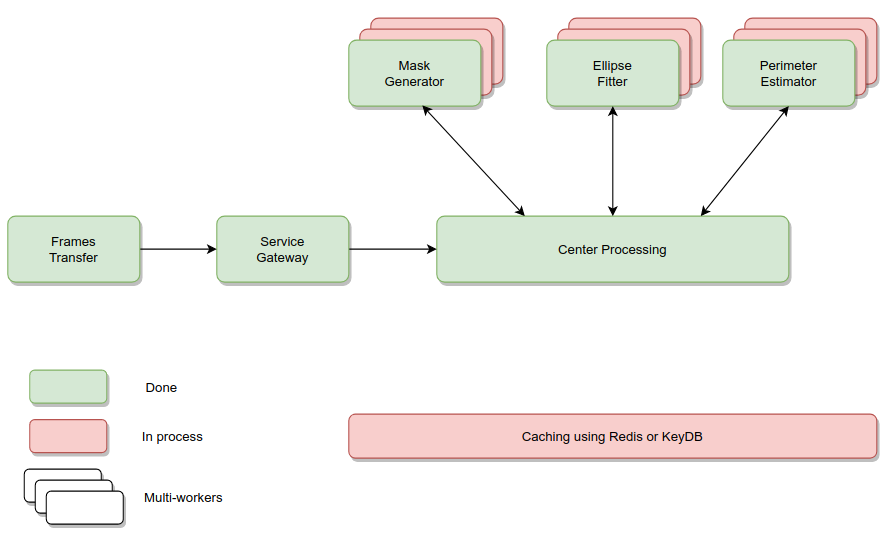
\includegraphics[width=0.9\textwidth]{./hinhanh/chap6/hc_system.png}}
		\caption{Proposed demo HC estimator system.}
		\label{fig:hc_system}
	\end{figure}

\section{Training Mask R-CNN}
\noindent
	
	In this research, we take advantage of a pre-trained model of Mask R-CNN and fine-tune it to for our problem instead of training the whole architecture of Mask R-CNN from scratch due to the lack of time and resources. Although Facebook's researchers published the official source code in 2018, we prefer using the unofficial one from Matterport Inc which was published in 2017 due to the majority of deep learning practitioner community (5k3 fork times compared to 9k6 ones, respectively). Further information, you can access the source code via this link \url{https://github.com/matterport/Mask_RCNN}.
	
\subsection{Configuration setting}
\noindent

	In the training phrase, focused on fine-tune several hyper-parameters that affected strongly for transfer learning technique. According to \cite{maskrcnn}, The default configuration was set based on Faster R-CNN due to its robustness on not only on detection task but also segmentation one. Look at Table \ref{table:hyperparameters} for more details about hyper-parameters.
	
	\begin{table}[H]
		\begin{tabularx}{1\textwidth} {
				| >{\raggedright\arraybackslash}X 
				| >{\raggedright\arraybackslash}X
				| >{\raggedright\arraybackslash}X 
				| >{\raggedright\arraybackslash}X
				| >{\raggedright\arraybackslash}X
				| >{\raggedright\arraybackslash}X
				| >{\raggedright\arraybackslash}X
				| >{\raggedright\arraybackslash}X
				| >{\raggedright\arraybackslash}X
				| >{\raggedright\arraybackslash}X
				| >{\raggedright\arraybackslash}X
				| >{\raggedright\arraybackslash}X
				| >{\raggedright\arraybackslash}X
				| >{\raggedright\arraybackslash}X  
				| >{\raggedright\arraybackslash}X | }
			\hline
			Model & Describe \\
			\hline
			IMAGE RESIZE MODE & Input image resizing. \\
			\hline
			STEPS PER EPOCH & Number of training steps per epoch. Don't set this too small to avoid spending a lot of time on validation stats. \\
			\hline
			VALIDATION STEPS & Number of validation steps to run at the end of every training epoch. A bigger number improves accuracy of validation stats, but slows down the training. \\
			\hline
			BACKBONE & Backbone network architecture. ResNet50 and ResNet101 are supported. \\
			\hline
			LEARNING RATE & Learning rate. \\
			\hline
			LEARNING MOMENTUM & Momentum \\
			\hline
			OPTIM & Optimization algorithm. \\
			\hline
			WEIGHT DECAY & Weight decay regularization. \\
			\hline
			LOSS WEIGHTS & Loss weights for more precise optimization. (Focus on desired loss) \\
			\hline
			
		\end{tabularx}
		\caption{Hyper-parameter description}
		\label{table:hyperparameters}
		
	\end{table}
	
	In Table \ref{table:hyperparameters}, we only list several hyper-parameters that are important in the fine-tune process. In addition, for more information of hyper-parameters, we recommend reader to read at \url{https://github.com/matterport/Mask_RCNN/blob/master/mrcnn/config.py}.
	
\subsection{Training}
\noindent

	As mentioned before, we used transfer learning technique to train Mask R-CNN. The dataset we used was described in \ref{subsection:dataset}. With a small pre-processing, we changed the annotation images and exported annotation's information (COCO's format) from it to fit Mask R-CNN's input requirement. In addition, we also applied data augmentation to increase the dataset size in order to avoid over-fitting problem. To be more precise, we created more images by:
	
	\begin{itemize}
		\item Flipping 50\% images vertically and horizontally, respectively.
		\item Rotating all images by 90, 180, and 270 degree.
		\item Multiplying images by a random value sampled uniformly from the interval [0.8, 1.5], making some images darker and others brighter.
		\item Blurring images using a gaussian kernel with a random standard deviation sampled uniformly (per image) from the interval [0.0, 5.0].
	\end{itemize}
	
	In the training process, we took advantages by using a pre-trained of Mask R-CNN trained on COCO dataset.... INTRODUCE the SCORE
	
	
	The result is illustrated in Table \ref{table:exp1}, \ref{table:exp2}. All of these configurations were set and fin-tuned based on \cite{maskrcnn} and \url{https://github.com/matterport/Mask_RCNN}.
	
	% Please add the following required packages to your document preamble:
	% \usepackage{multirow}
	% \usepackage{longtable}
	% Note: It may be necessary to compile the document several times to get a multi-page table to line up properly

	\begin{longtable}[c]{|c|l|l|l|l|l|}
		\hline
		& \multicolumn{1}{c|}{\textbf{Test 1}} & \multicolumn{1}{c|}{\textbf{Test 2}} & \multicolumn{1}{c|}{\textbf{Test 3}} & \multicolumn{1}{c|}{\textbf{Test 4}} & \multicolumn{1}{c|}{\textbf{Test 5}} \\ \hline
		\endfirsthead
		%
		\multicolumn{6}{c}%
		{{\bfseries Table \thetable\ continued from previous page}} \\
		\endhead
		%
		\textbf{Backbone} & Resnet50 & Resnet50 & Resnet101 & Resnet101 & Resnet101 \\ \hline
		\textbf{Optimizer} & SGD & Adam & SGD & Adam & SGD \\ \hline
		\textbf{Learning rate} & 0.001 & 0.001 & 0.001 & 0.001 & 0.0001 \\ \hline
		\textbf{Weight decay} & 0.0005 & 0.0005 & 0.0005 & 0.0005 & 0.0005 \\ \hline
		\textbf{Momentum} & 0.9 & 0.9 & 0.9 & 0.9 & 0.9 \\ \hline
		\textbf{Epoch} & 20 & 20 & 20 & 20 & 30 \\ \hline
		\textbf{Train - Val step} & 150 - 50 & 150 - 50 & 150 - 50 & 150 - 50 & 150 - 50 \\ \hline
		\textbf{Detection min confidence} & 0 & 0 & 0.9 & 0.9 & 0.9 \\ \hline
		\textbf{Detection NMS threshold} & 0.9 & 0.9 & 0.9 & 0.9 & 0.9 \\ \hline
		\multirow{2}{*}{\textbf{RPN anchor scale}} & \multirow{2}{*}{16, 32, 64, 128, 256} & \multirow{2}{*}{16, 32, 64, 128, 256} & \multirow{2}{*}{16, 32, 64, 128, 256} & \multirow{2}{*}{16, 32, 64, 128, 256} & \multirow{2}{*}{16, 32, 64, 128, 256} \\
		&  &  &  &  &  \\ \hline
		\textbf{Resize mode} & square & square & square & square & square \\ \hline
		\multirow{6}{*}{\textbf{Loss weight}} & rpn class loss: 1.0, & rpn class loss: 1.0, & rpn class loss: 1.0, & rpn class loss: 1.0, & rpn class loss: 1.0, \\ \cline{2-6} 
		& rpn bbox loss: 1.0, & rpn bbox loss: 1.0, & rpn bbox loss: 1.0, & rpn bbox loss: 1.0, & rpn bbox loss: 1.0, \\ \cline{2-6} 
		& mrcnn class loss: 1.0, & mrcnn class loss: 1.0, & mrcnn class loss: 1.0, & mrcnn class loss: 1.0, & mrcnn class loss: 1.0, \\ \cline{2-6} 
		& mrcnn bbox loss: 1.0, & mrcnn bbox loss: 1.0, & mrcnn bbox loss: 1.0, & mrcnn bbox loss: 1.0, & mrcnn bbox loss: 1.0, \\ \cline{2-6} 
		& \multirow{2}{*}{mrcnn mask loss: 3.0} & \multirow{2}{*}{mrcnn mask loss: 3.0} & \multirow{2}{*}{mrcnn mask loss: 3.0} & \multirow{2}{*}{mrcnn mask loss: 3.0} & \multirow{2}{*}{mrcnn mask loss: 3.0} \\
		&  &  &  &  &  \\ \hline
		\textbf{mAP} & 0.511111 & 0.822222222 & 0.977777777 & 0.0 & 0.9419753 \\ \hline
		\textbf{mAR} & 0.533333 & 0.837037037 & 0.977777777 & 0.0 & 0.9703703 \\ \hline
		\textbf{NOTE} & SGD train faster but trade off accuracy & Adam shows better much results but training time is slower than SGD & SGD shows it is better in using resnet101 & Training loss went NaN value because lr is high &  \\ \hline
	
	\caption{Experiment results}
	\label{table:exp1}
	\end{longtable}

	
	% Please add the following required packages to your document preamble:
	% \usepackage{multirow}
	% \usepackage{longtable}
	% Note: It may be necessary to compile the document several times to get a multi-page table to line up properly
	\begin{longtable}[c]{|c|l|l|l|l|l|}
		\hline
		& \multicolumn{1}{c|}{\textbf{Test 6}} & \multicolumn{1}{c|}{\textbf{Test 7}} & \multicolumn{1}{c|}{\textbf{Test 8}} & \multicolumn{1}{c|}{\textbf{Test 9}} & \multicolumn{1}{c|}{\textbf{Test 10}} \\ \hline
		\endhead
		%
		\textbf{Backbone} & Resnet50 & Resnet50 & Resnet50 & Resnet101 & Resnet101 \\ \hline
		\textbf{Optimizer} & Adam & Adam & SGD & SGD & Adam \\ \hline
		\textbf{Learning rate} & 0.0001 & 0.0001 & 0.001 & 0.001 & 0.0001 \\ \hline
		\textbf{Weight decay} & 5,00E-05 & 5,00E-05 & 0.0005 & 0.0005 & 0.0005 \\ \hline
		\textbf{Momentum} & 0.9 & 0.9 & 0.9 & 0.9 & 0.9 \\ \hline
		\textbf{Epoch} & 30 & 30 & 30 & 30 & 30 \\ \hline
		\textbf{Train - Val step} & 150 - 50 & 150-50 & 150 - 50 & 150 - 50 & 150 - 50 \\ \hline
		\textbf{Detection min confidence} & 0.7 & 0.7 & 0.7 & 0.7 & 0.9 \\ \hline
		\textbf{Detection NMS threshold} & 0.7 & 0.7 & 0.7 & 0.7 & 0.9 \\ \hline
		\multirow{2}{*}{\textbf{RPN anchor scale}} & \multirow{2}{*}{16, 32, 64, 128, 256} & \multirow{2}{*}{16, 32, 64, 128, 256} & \multirow{2}{*}{16, 32, 64, 128, 256} & \multirow{2}{*}{16, 32, 64, 128, 256} & \multirow{2}{*}{16, 32, 64, 128, 256} \\
		&  &  &  &  &  \\ \hline
		\textbf{Resize mode} & square & square & square & square & square \\ \hline
		\multirow{6}{*}{\textbf{Loss weight}} & rpn class loss: 1.0, & rpn class loss: 1.0, & rpn class loss: 1.0, & rpn class loss: 1.0, & rpn class loss: 1.0, \\ \cline{2-6} 
		& rpn bbox loss: 1.0, & rpn bbox loss: 1.0, & rpn bbox loss: 1.0, & rpn bbox loss: 1.0, & rpn bbox loss: 1.0, \\ \cline{2-6} 
		& mrcnn class loss: 1.0, & mrcnn class loss: 1.0, & mrcnn class loss: 1.0, & mrcnn class loss: 1.0, & mrcnn class loss: 1.0, \\ \cline{2-6} 
		& mrcnn bbox loss: 1.0, & mrcnn bbox loss: 1.0, & mrcnn bbox loss: 1.0, & mrcnn bbox loss: 1.0, & mrcnn bbox loss: 1.0, \\ \cline{2-6} 
		& \multirow{2}{*}{mrcnn mask loss: 1.0} & \multirow{2}{*}{mrcnn mask loss: 1.0} & \multirow{2}{*}{mrcnn mask loss: 1.0} & \multirow{2}{*}{mrcnn mask loss: 1.0} & \multirow{2}{*}{mrcnn mask loss: 1.0} \\
		&  &  &  &  &  \\ \hline
		\textbf{mAP} & 0.43703703703 & 0.955555555556 & 0.16296296298 & 0.9407407408 &  \\ \hline
		\textbf{mAR} & 0.62222222222 & 0.970370370370 & 0.16296296298 & 0.9851851852 &  \\ \hline
		\textbf{NOTE} & ??? & ??? & SGD not works well with resnet50 &  &  \\ \hline
	
	\caption{Experiment results}
	\label{table:exp2}
	\end{longtable}
	
	Firstly, we started our training process with "Test 1" and "Test 2" in order to find out which optimizer was better than the other. In general, it is noticeable that Adam optimizer converged faster than SGD one. Moreover, model with Adam optimizer showed a much better mAP and mAR compared to model with SGD. 
	
 	In "Test 3, 4", we change the backbone from ResNet50 to ResNet101 to see could we actually improve the model by going deeper? And the results were quite significant. In "Test 3", with ResNet101, we improved the model mAP and mAR from ~0.5 to 0.97777 which was the highest score in lots of experiments we had proceeded. However, loss value of "Test 4" went to NaN due to the high learning rate which showed Adam optimizer was quite sensitive to the high learning rate. Therefore, in "Test 5" we decreased the learning rate to 0.0001, as the result, the model showed a better result (yet, its mAP and mAR were still low). Consequently, we could boost mAP and mAR score to 0.9419753 and 0.9703703, respectively.
	
	Although, Adam optimizer with ResNet50 backbone showed a remarkable result, SGD optimizer with ResNet101 backbone illustrated the highest results in "Test 3" and "Test 9" with mAP and mAR are (0.977777, 0.977777) and (0.9407408, 0.9851852), respectively.
	